\section{Security Validation \& Testing}

\subsection{Scope and Methodology}
The security validation of the CFI-Care platform was conducted using a dual-layer approach to ensure both architectural integrity and infrastructure resilience.
\begin{itemize}
    \item \textbf{Application-Layer Logic}: Automated unit tests (Jest/Supertest) were employed to validate the Authorization and Authentication middleware, 
    with a methodology focused on negative testing, ensuring the system enforces security policies even when presented with incorrect or even malicious input
    \item \textbf{Infrastructure Vulnerability Assessment}: A web-based vulnerability scan (Tenable Nessus) and directory brute-forcing (Dirb) were conducted to identify configuration and exposure risks.
    \item \textbf{Perimeter and Integrity Testing}: Manual request manipulation (Burp Suite) was utilized to verify the robustness of OIDC/PKCE flows, session management and XSRF protection mechanisms
\end{itemize}

\subsection{Validation Results}
Table~\ref{tab:security_validation} synthesizes the goals of automated scans and manual logic verification

\begin{table}[ht]
    \centering
    \caption{Security Validation and Penetration Testing Goals}
    \label{tab:security_validation}
    \renewcommand{\arraystretch}{1.3}
    \begin{tabular}{|p{0.25\linewidth}|p{0.2\linewidth}|p{0.35\linewidth}|}
        \hline
        \textbf{Test Scenario} & \textbf{Validation Method} & \textbf{Observation} \\ \hline
        OIDC/PKCE Gateway	& Unit Test (Jest) & Validates state logic \& profile fetching	\\ \hline
        Consent Handshake & Unit Test (Jest) & validates OTP logic \\ \hline
        API Transport & Unit Test (Jest) & Validates the mitigation of unsigned/malformed bearer tokens \\ \hline
        % Auth/Me Endpoint & Unit Test (Jest) & Rejects anonymous requests with 401 \\ \hline
        Cookie Attributes & Nessus Scan & HttpOnly/Secure flags verified \\ \hline
        Directory Indexing & Dirb Brute-force & Verify /auth paths are throttled (429 limited) \\ \hline
        % PKCE Flow & Burp Suite & State parameters validated \\ \hline
        Request State Integrity & Burp Suite & Validates mandatory XSRF-TOKEN header \\ \hline
        % Scope Enforcement & Unit Test (Jest) & Mismatched patient IDs trigger 403 \\ \hline
    \end{tabular}
\end{table}

\subsubsection{Security Evolution}
A comparison between the baseline assessment conducted in March 2026 (displayed in Figs~\ref{fig:init-nessus-vul} and \ref{fig:init-nessus-vul2}) and the final validation in June 2026 (Displayed in Fig~\ref{fig:final-nessus}) shows a maturation of the CFI-Care platform's security posture; 
initial findings identified missing security headers (HSTS) and permissive cookie attributes, which were remediated through Nginx configuration hardening. 
Furthermore, after the initial Burpsuite test highlighted the lack of a XSRF token, we implemented strict header validation (Fig~\ref{fig:xsrf-verification}), which has mitigated risks associated with cross-site request forgery.


\begin{figure}[H]
    \centering
    \fbox{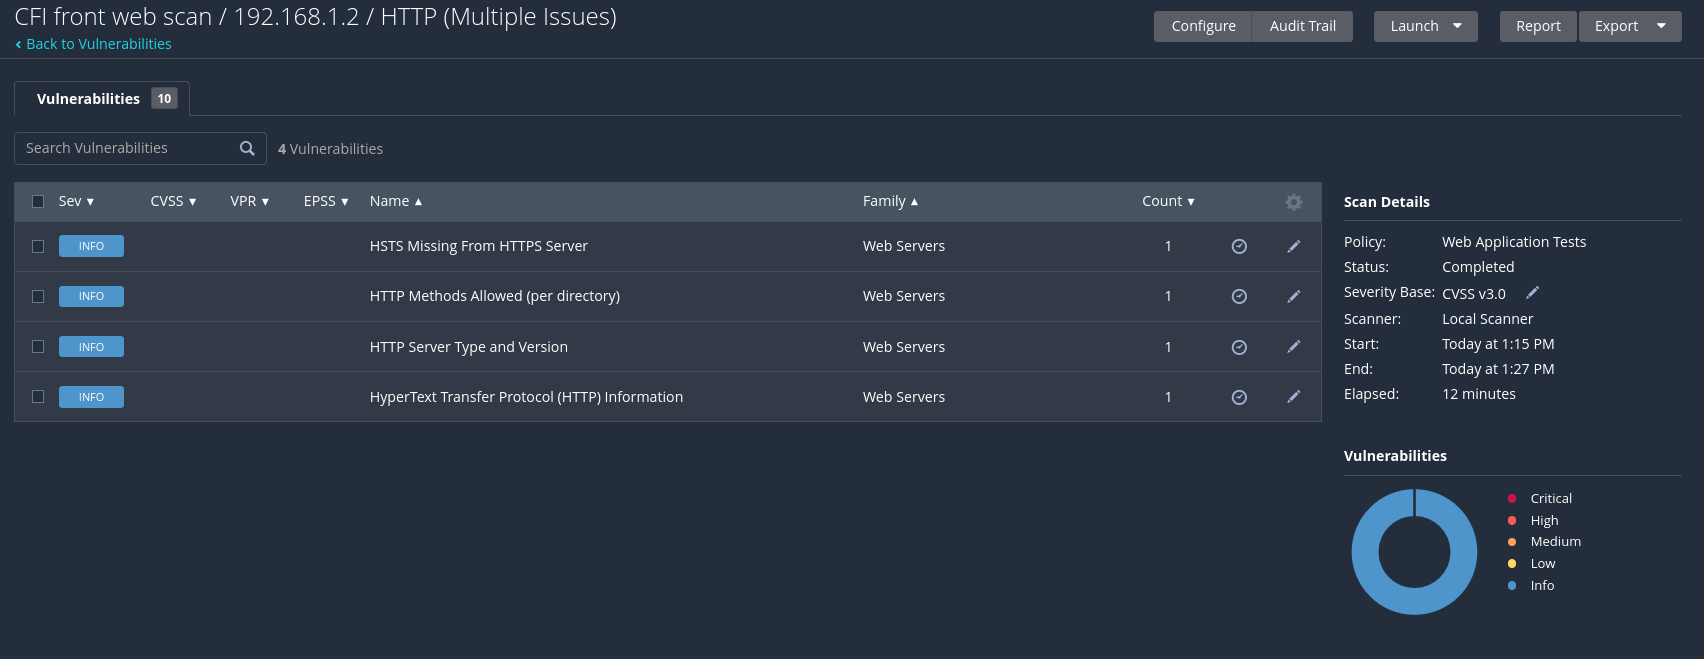
\includegraphics[width=0.8\textwidth]{Testing/Images/security/http.png}}
    \caption{Initial Nessus Vulnerability Scan highlights for the browser side system running on the host}
    \label{fig:init-nessus-vul}
\end{figure}

\begin{figure}[H]
    \centering
    \fbox{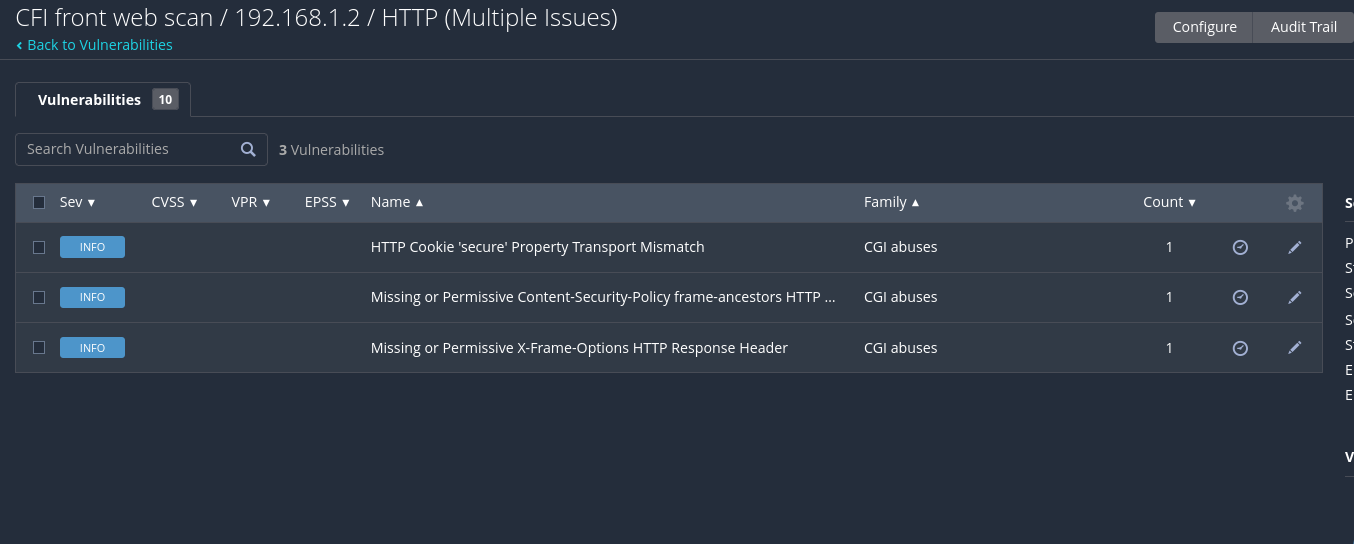
\includegraphics[width=0.8\textwidth]{Testing/Images/security/http2.png}}
    \caption{Initial Nessus Vulnerability Scan highlights for the browser side system running on the host}
    \label{fig:init-nessus-vul2}
\end{figure}

\begin{figure}[H]
\centering
\fbox{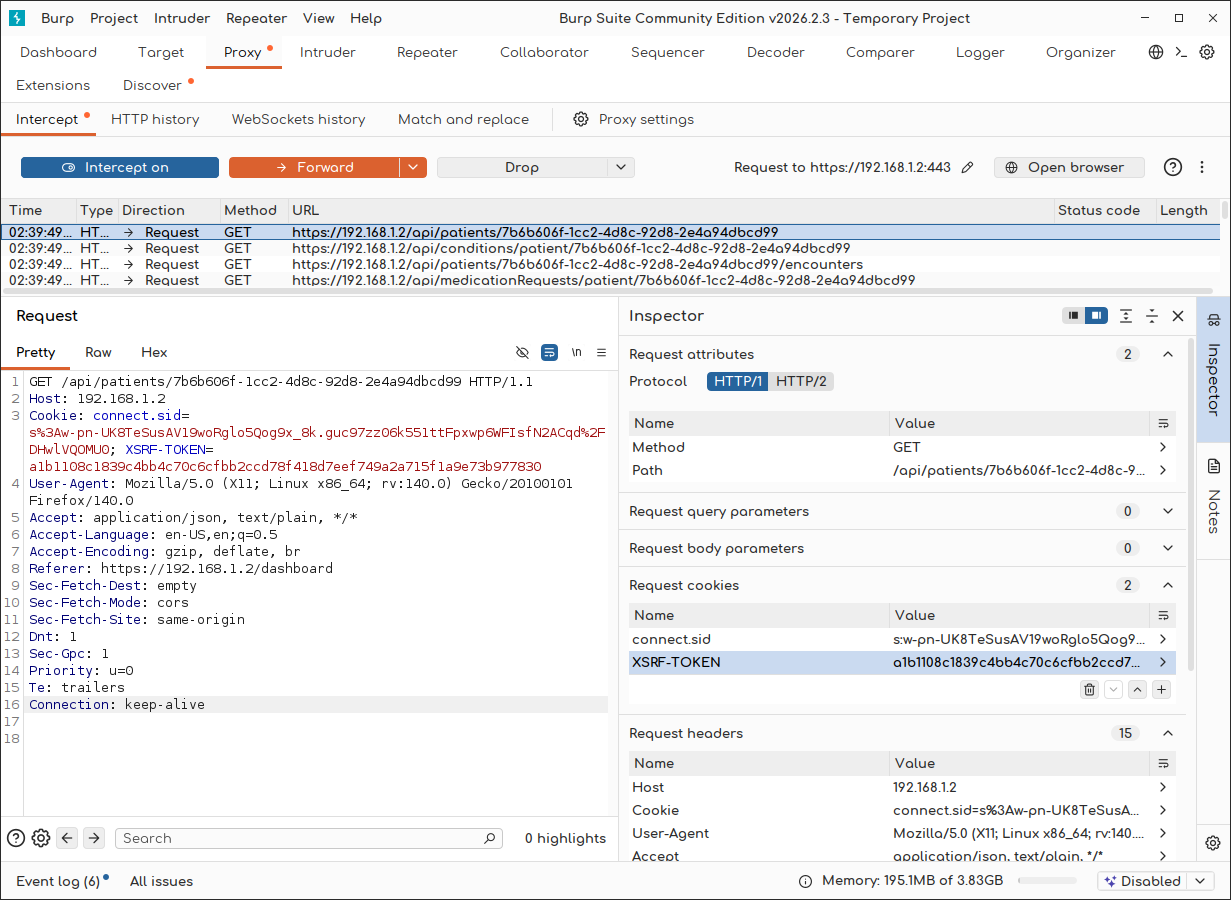
\includegraphics[width=0.8\textwidth]{Testing/Images/security/xsrf.png}}
\caption{Burp Suite Interception: Verification of XSRF token enforcement on API requests.}
\label{fig:xsrf-verification}
\end{figure}


\subsection{Infrastructure Hardening (Nessus Assessment)}
The Nessus web scan identified the platform's footprint, including the detection of the Nginx web server. 
The scan highlighted informational findings regarding server-identifying headers and cookie attribute enforcement.
\begin{itemize}
    \item \textbf{Remediation:} Nginx configuration was hardened to strip server-identifying headers and enforce \texttt{HttpOnly} and \texttt{Secure} attributes across all domain-level cookies.
\end{itemize}


\begin{figure}[H]
    \centering
    \fbox{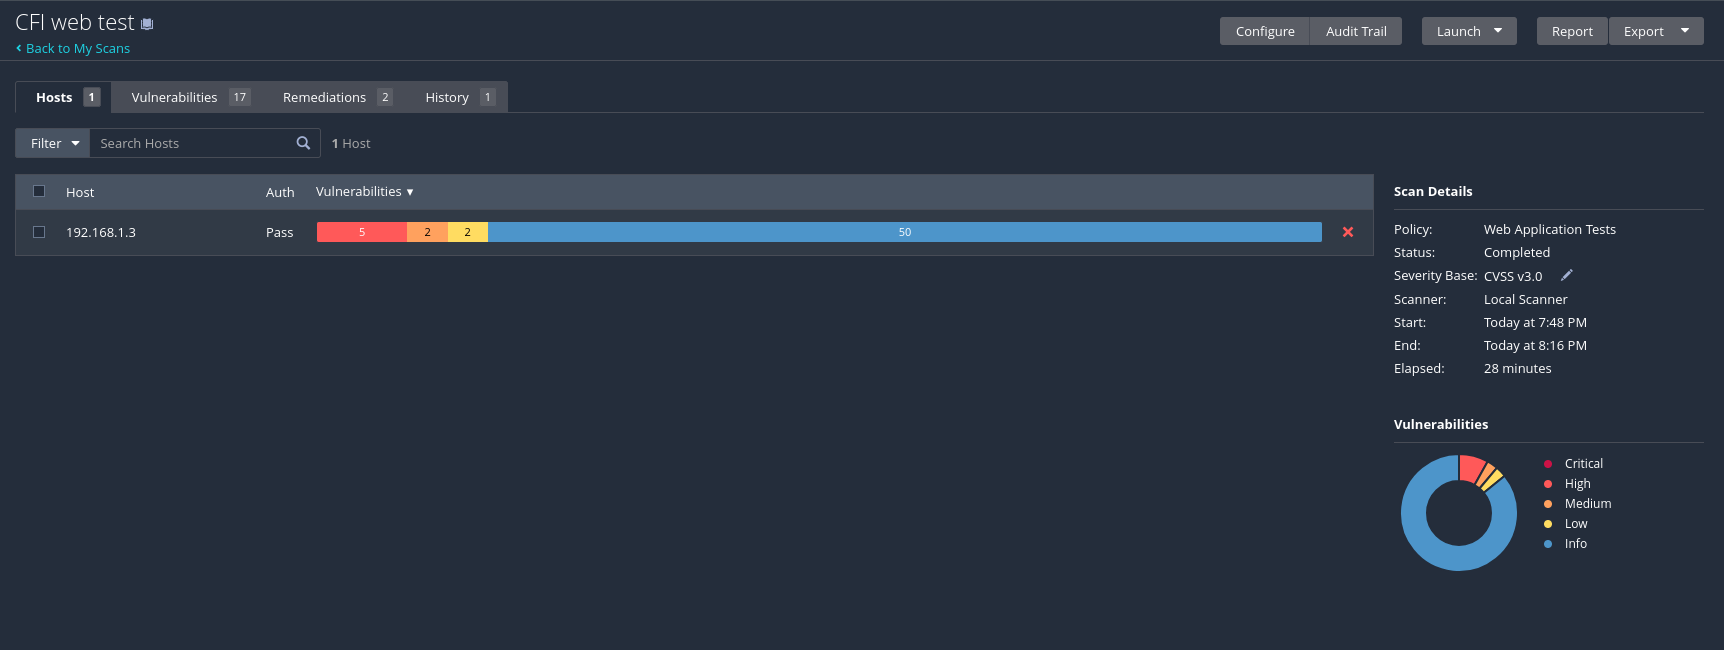
\includegraphics[width=0.8\textwidth]{Testing/Images/security/nessus_report_summary.png}}
    \caption{Final Nessus Vulnerability Scan: Summary for the browser side system running on the host}
    \label{fig:final-nessus}
\end{figure}

\begin{figure}[H]
    \centering
    \fbox{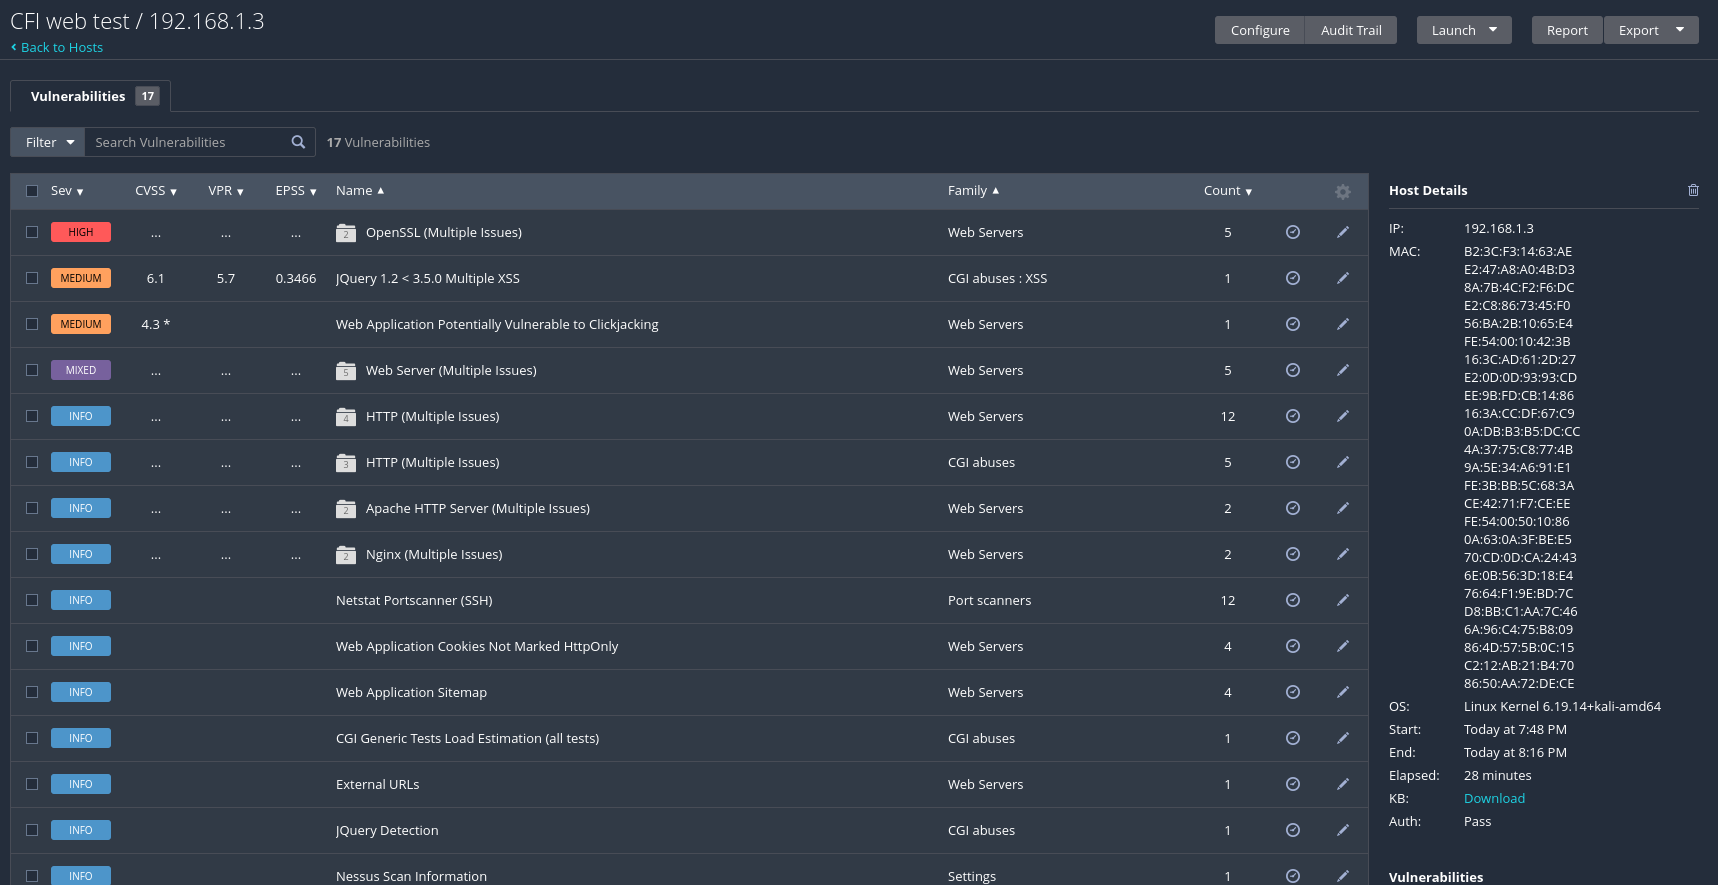
\includegraphics[width=0.8\textwidth]{Testing/Images/security/nessus_vulnerabilities_page.png}}
    \caption{Nessus Vulnerability Scan: Complete removal of actionable security risk flags}
\end{figure}


\subsection{Manual Penetration Testing (Burp Suite)}
Manual assessment verified the OIDC/PKCE callback flow by intercepting the token exchange via Burp Suite, where the system's ability to maintain state consistency was validated. 
These tests confirmed that parameter manipulation resulted in immediate rejection, preventing potential CSRF or code injection.

\begin{figure}[H]
    \centering
    \fbox{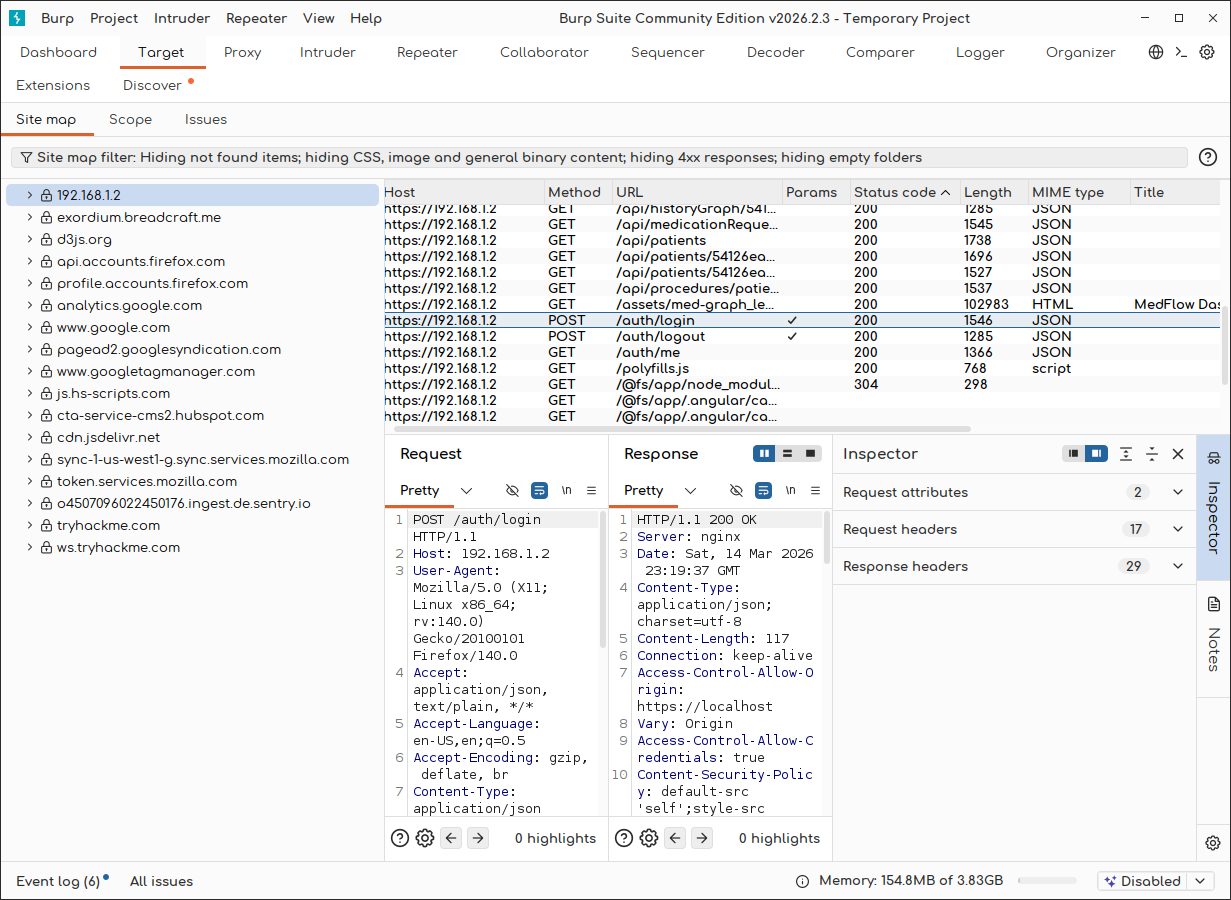
\includegraphics[width=0.8\textwidth]{Testing/Images/security/burprep1.png}}
    \caption{Burp Suite Interception: verification of protected authentication routes}
\end{figure}

\begin{figure}[H]
    \centering
    \fbox{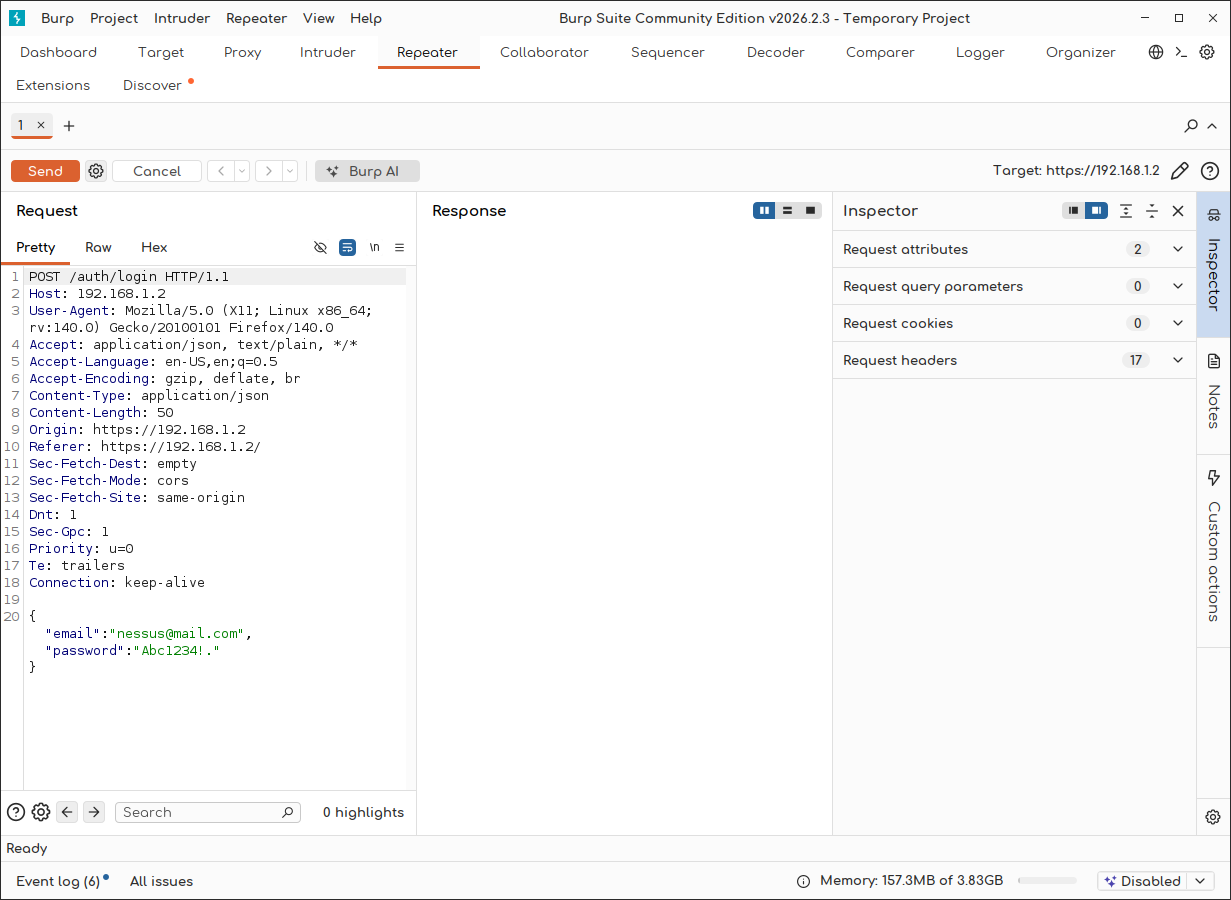
\includegraphics[width=0.8\textwidth]{Testing/Images/security/burprep2.png}}
    \caption{Burp Suite Interception: Manual Credential Testing}
\end{figure}

\begin{figure}[H]
    \centering
    \fbox{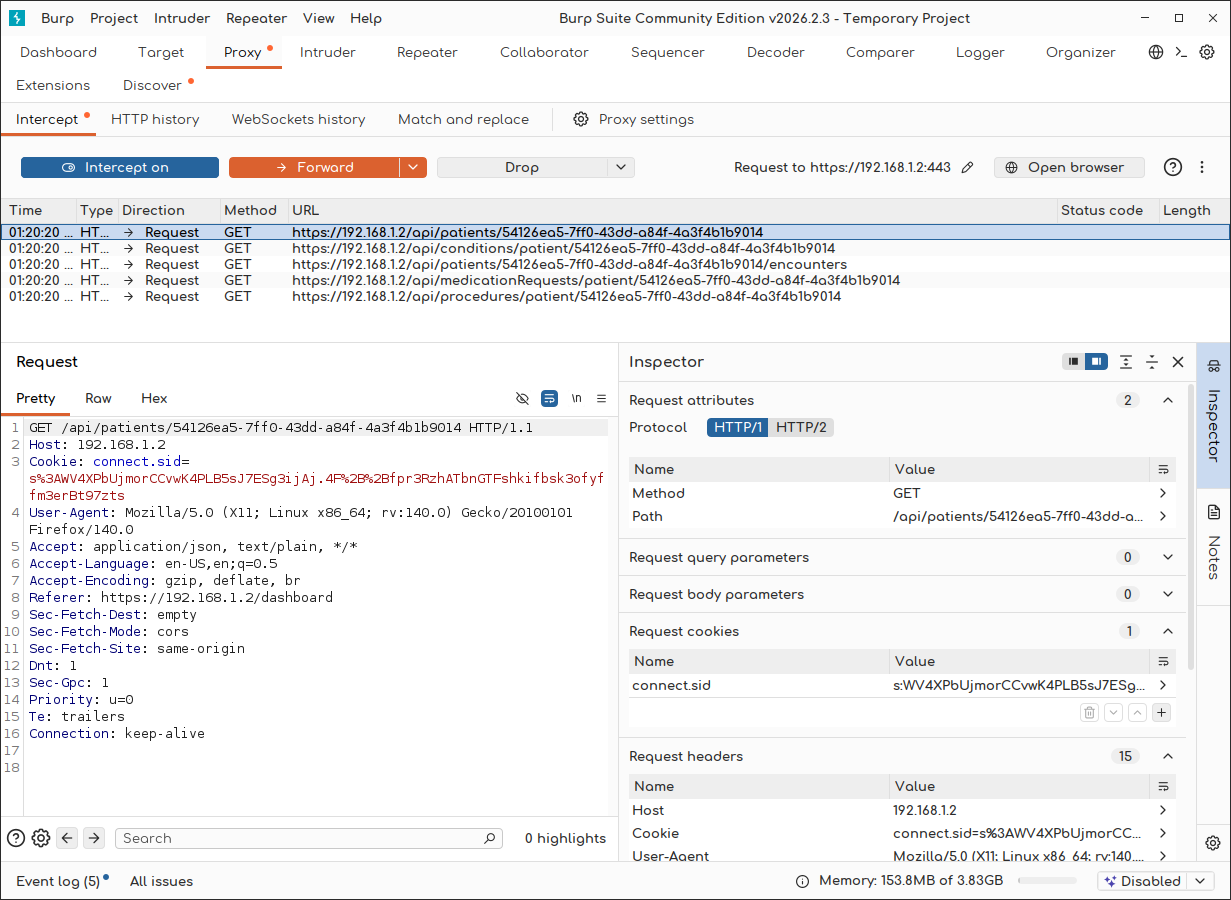
\includegraphics[width=0.8\textwidth]{Testing/Images/security/burp6.png}}
    \caption{Burp Suite Interception: Auth State Verification}
\end{figure}

\subsection{Logical Security Coverage}
The application logic was validated through 39 unit tests, they're categorized by their specific security function:

\begin{itemize}
    \item \textbf{Identity \& Session Handshaking:} 10 tests (AUTH-001 to AUTH-008) validate the OIDC/PKCE handshake, including state parameter consistency, secure token exchange, and dynamic session initialization
    \item \textbf{Consent \& OTP Handshakes:} 15 tests (HANDSHAKE-001 to HANDSHAKE-014) verify the consent creation logic
    \item \textbf{API Authentication \& JWT Integrity}: 9 tests (SEC-API-001 to SEC-API-011) verify the rejection of malformed or unsigned bearer tokens and ensure that only allowlisted clients (e.g., the Provisioner Client) can access sensitive administrative endpoints
    \item \textbf{Resource Scope Enforcement}: 5 tests (SEC-SCOPE-001 to SEC-SCOPE-005) enforce SMART-on-FHIR specifications, validating patient resource targets against current token claims to guarantee data isolation. 
\end{itemize}

Beyond automated logic validation, manual interception was used to confirm that the session-level authorization remains bound to specific resource scopes, Fig~\ref{fig:burp-cookie-auth} illustrates the inspection of encrypted session cookies and their corresponding authorization headers during a live state transition. 
Finally, Fig~\ref{fig:burp-scope-isolation} demonstrates the verification of scoped data isolation, confirming that the session maintains access only to the FHIR resources explicitly granted during the OIDC handshake, effectively preventing cross-tenant data leakage at the browser level.

\begin{figure}[H]
    \centering
    \fbox{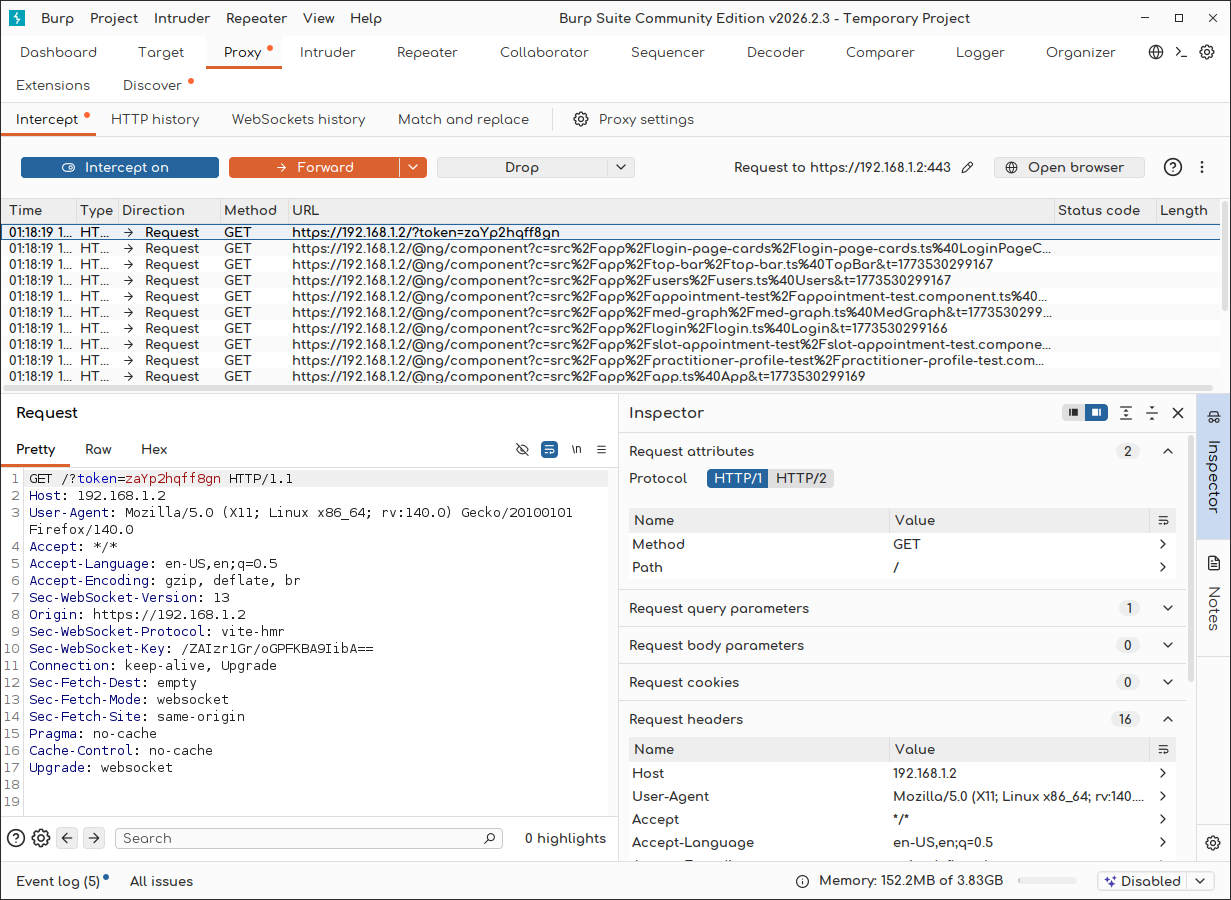
\includegraphics[width=0.8\textwidth]{Testing/Images/security/burp4.png}}
    \caption{Burp Suite Interception: Inspection of encrypted session cookies and auth header integrity}
    \label{fig:burp-cookie-auth}
\end{figure}

\begin{figure}[H]
    \centering
    \fbox{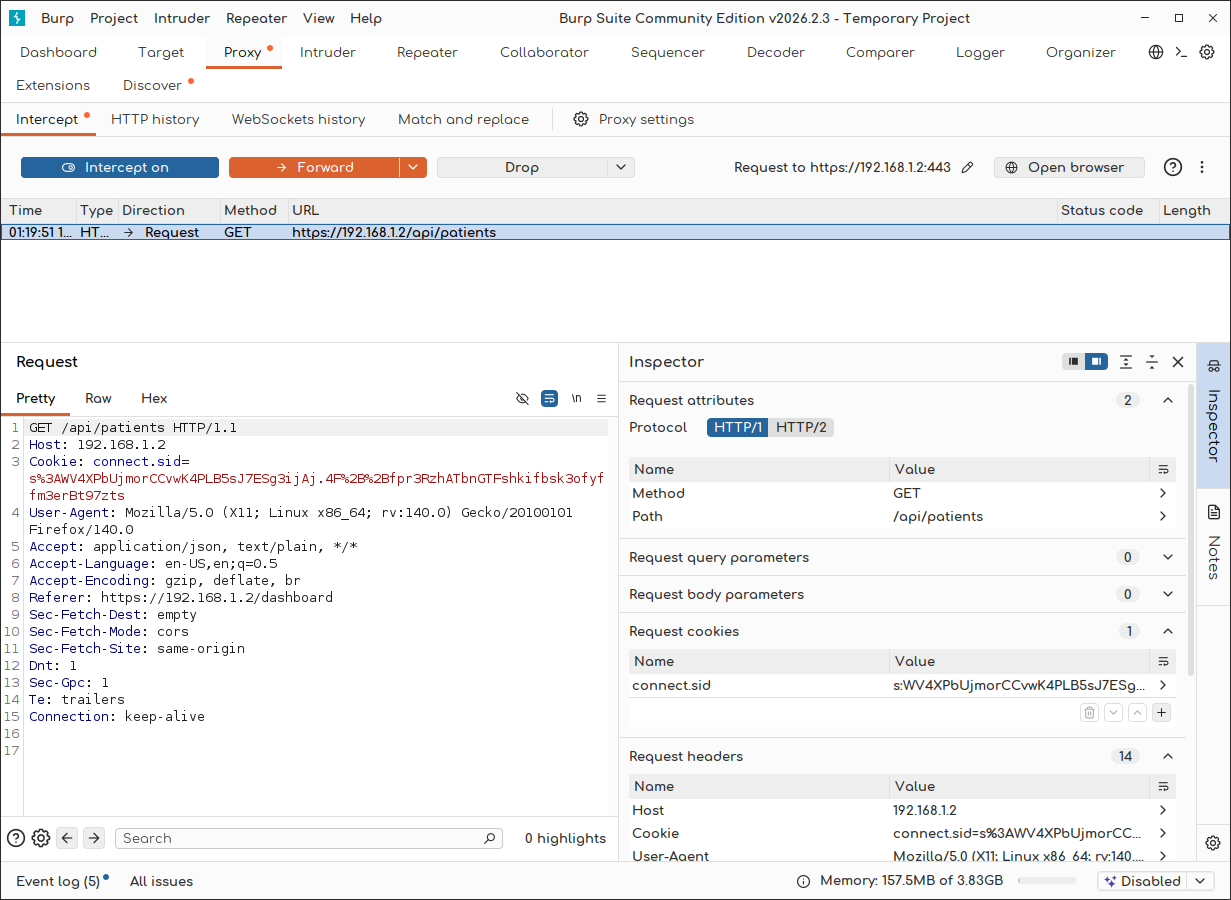
\includegraphics[width=0.8\textwidth]{Testing/Images/security/burp5.png}}
    \caption{Burp Suite Interception: Verification of scoped patient data isolation within an active session}
    \label{fig:burp-scope-isolation}
\end{figure}
